\clearpage{\pagestyle{empty}\cleardoublepage}
\chapter{Implementazione}

\section{Le scelte di base}

La primissima scelta che ci si pone davanti è chiaramente quella sul linguaggio di programmazione da adottare. Siccome tutte le premesse fatte hanno come denominatore comune la \emph{velocità} nell'esecuzione delle varie operazioni, si sono scelti il C e il C++, che essendo linguaggi compilati offrono sicuramente prestazioni migliori rispetto a linguaggi interpretati. Inoltre, la prerogativa di realizzare un software libero, suggerisce di sviluppare il programma su Linux, il sistema operativo libero per antonomasia.

Facciamo un piccolo riassunto di cosa macroscopicamente il firewall debba fare. Per prima cosa, bisogna catturare il pacchetto dalla scheda di rete, successivamente processarlo, salvando le informazioni utili e analizzandolo completamente per riconoscerne il protocollo applicativo, ed infine, decidere se e quando trasmetterlo sull'altro lato.

Per rispondere alla prima esigenza è stata naturalmente presa in considerazione la classica libreria PCAP \cite{pcap,pcap2}. Purtroppo tale libreria è stata ideata in un momento in cui le schede di rete erano decisamente più lente, quindi risulta inadeguata ai nostri scopi. Così si è optato per l'utilizzo della libreria PF\_RING \cite{pfring}, che garantisce un rate di cattura intorno al Gigabit/s.

Per processare il pacchetto sono necessarie due operazioni. La prima consiste nel salvare in un'apposita struttura dati le varie informazioni che via via si ricavano dai pacchetti catturati. Dal corso di Algoritmica, risulta subito chiaro come l'utilizzo di una hash table di dimensione statiche (per evitare il blocco dell'esecuzione per attendere il ridimensionamento) con collisioni gestite a lista di trabocco sia la soluzione migliore in termini di prestazioni. La seconda, di importanza centrale nel firewall, analizza il pacchetto ricevuto fino al payload trasportato. Pochissime librerie open source consentono di eseguire il DPI efficientemente. La libreria L7-Filter \cite{l7filter}, eseguendo il confronto per pattern matching di espressioni regolari, è piuttosto lenta, e soffre dei problemi legati ai falsi positivi. Quindi la scelta è ricaduta sulla libreria nDPI \cite{ndpi}, che utilizzando semplici funzioni C permette prestazioni superiori e una probabilità di errore nel riconoscimento del protocollo applicativo praticamente nulla.

Infine il firewall si trova a dover affrontare una scelta, se far proseguire il pacchetto verso la destinazione o meno. A questo punto si consultano le regole impostate dall'utente salvate anch'esse in un'apposita struttura dati. In questo caso, la tabella hash non è la soluzione indicata, in quanto comunque le regole vanno scelte anche in base al prefisso più lungo comune sull'indirizzo IP. Sempre dal corso di Algoritmica, la miglior struttura dati da usare in questo caso risulta essere un albero binario sui bit dell'indirizzo.

\subsection{I PF\_RING}

I PF\_RING \cite{pfring} non sono altro che un nuovo tipo di socket di rete in grado di catturare pacchetti dalla scheda di rete e portarli in spazio utente, riuscendo a gestire traffico a velocità anche intorno ai 10 Gigabit/s.

L'idea alla base di questa tecnologia è quella di utilizzare un buffer circolare (detto \emph{ring}) dove salvare i pacchetti ricevuti dalla scheda e quindi passare all'applicazione il puntatore al pacchetto tramite una chiamata alla system call mmap(), mappando cioè in memoria virtuale del programma tale indirizzo. Questo è ottenuto attraverso due strati di polling. Uno posto tra la scheda e il \emph{ring}, l'altro tra il \emph{ring} e l'applicazione. Il primo sfrutta le NAPI (o New API) \cite{napi}, delle tecniche che consentono di mitigare l'effetto degli interrupt del device sul kernel di Linux, potendo richiederne l'intervento dopo un certo numero di pacchetti ricevuti (infatti il comportamento standard impone che ogni volta che la scheda riceva un pacchetto, mandi un \emph{interrupt} al sistema operativo per richiederne l'elaborazione, interrompendone quindi continuamente l'esecuzione). Il secondo sfrutta un semplice meccanismo di polling dei vari \emph{ring}, al fine di trovare nuovi pacchetti da portare in user-space tramite la funzione mmap().

Una peculiarità è l'indipendenza dallo specifico driver della scheda di rete. Vi sono tuttavia una serie di driver riscritti per supportare la vera potenza dei PF\_RING, i DNA driver.

Il DNA (\emph{Direct NIC Access}) \cite{pfringdna} consente di accedere direttamente alla memoria della scheda di rete, mappandone gli indirizzi. Potendo fare questo tipo di accesso ai vari registri del device, non c'è più bisogno di utilizzare la CPU. Si ha un grande miglioramento delle performance dovuto sia al risparmio dei cicli di clock spesi per salvare il pacchetto nel \emph{ring}, che quelli spesi per interrogare il device sui nuovi pacchetti ricevuti. Ciò che viene sfruttato ora, è la NPU (\emph{Network Processing Unit}), al fine di portare il pacchetto dalla scheda al \emph{ring} aperto in modalità DMA (\emph{Direct Memory Access}). Il risultato di tutto questo, è la possibilità di inviare e ricevere pacchetti di qualsiasi grandezza alla stessa velocità supportata dalla scheda.

\begin{figure}[htbp]
\begin{center}
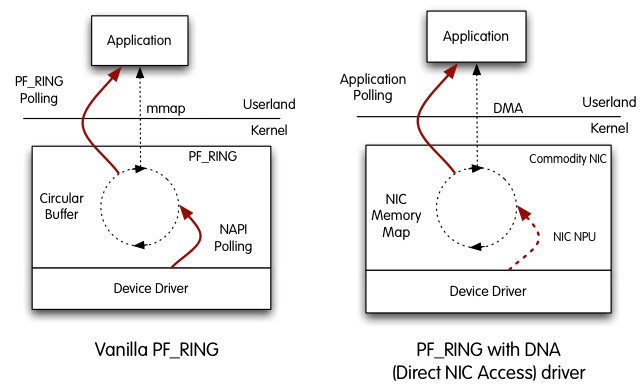
\includegraphics[scale=0.5]{img/PF_Ring_DNA.png}
\caption{Confronto tra le due realizzazioni}\label{PFRingDNA}
\end{center}
\end{figure}

\subsection{La libreria nDPI}

Per affrontare il problema cardine del nuovo concetto di firewall, ovvero l'analisi approfondita dei pacchetti, è stata scelta la libreria nDPI \cite{ndpi}, scritta in C, e nata dalle ceneri di un altro progetto open source abbandonato, \emph{OpenDPI}, del quale sul web rimangono pochissime tracce.

Data la sua natura, oltre a ottime performance, garantisce una quasi inesistente possibilità di avere dei falsi positivi e negativi, caratteristiche davvero importanti per una libreria che si occupa del DPI.

Questa libreria permette di esaminare singoli pacchetti, tenendo conto anche delle informazioni precedentemente salvate su quel flusso (reperibili dalla hash table), al fine di ottenere un codice identificativo del protocollo applicativo. Se nessuna corrispondenza venisse trovata col primo pacchetto, si dovrebbe procedere con i successivi che via via arriveranno al sistema, al fine di trovarne il servizio effettivamente trasportato.

Purtroppo non è sempre possibile risalire al protocollo applicativo (ad esempio perché tale protocollo non è supportato dalla libreria, oppure perché è cambiato nel tempo). Quindi conviene provare ad identificare il flusso solo per un numero di pacchetti limitato, per non incorrere in inutili prove, costose in termini di tempo. Dopodiché, se non si trovasse il servizio trasportato, tale flusso rimarrebbe non riconosciuto.

I protocolli riconosciuti sono comunque circa 150 e comprendono servizi usati per le funzioni di connettività e utilità (come DNS, DHCP, TELNET, NETBIOS, \dots), mail (POP3, SMTP, IMAP, GMAIL, \dots), web (HTTP, Flash, QuickTime, FaceBook, Twitter, YouTube, \dots), giochi e simili (Quake, SecondLife, \dots), trasferimento file (FTP, EDonkey, BitTorrent, \dots), \dots . Insomma, un parco protocolli davvero completo in grado di spaziare tra i vari settori d'uso di Internet.

Per eseguire le sue operazioni, tutte le chiamate a funzione fanno capo ad un'unica struttura principale condivisa che ha al suo interno, fra le altre cose, un buffer di funzioni. Queste sono quelle che realmente provano a stabilire se un dato pacchetto, passato come argomento, appartiene ad un certo protocollo applicativo.

Risulta quindi evidente come questa libreria sia facilmente estendibile. Basterà aggiungere a tale buffer una nuova funzione per identificare un nuovo protocollo (codificato da un numero univoco rispetto agli altri), per avere un nuovo servizio supportato.

Anche questo aspetto di flessibilità e facilità nell'aggiornamento è stato determinante per la scelta di questa libreria.

\subsection{L'architettura del sistema}

\begin{figure}[htbp]
\begin{center}
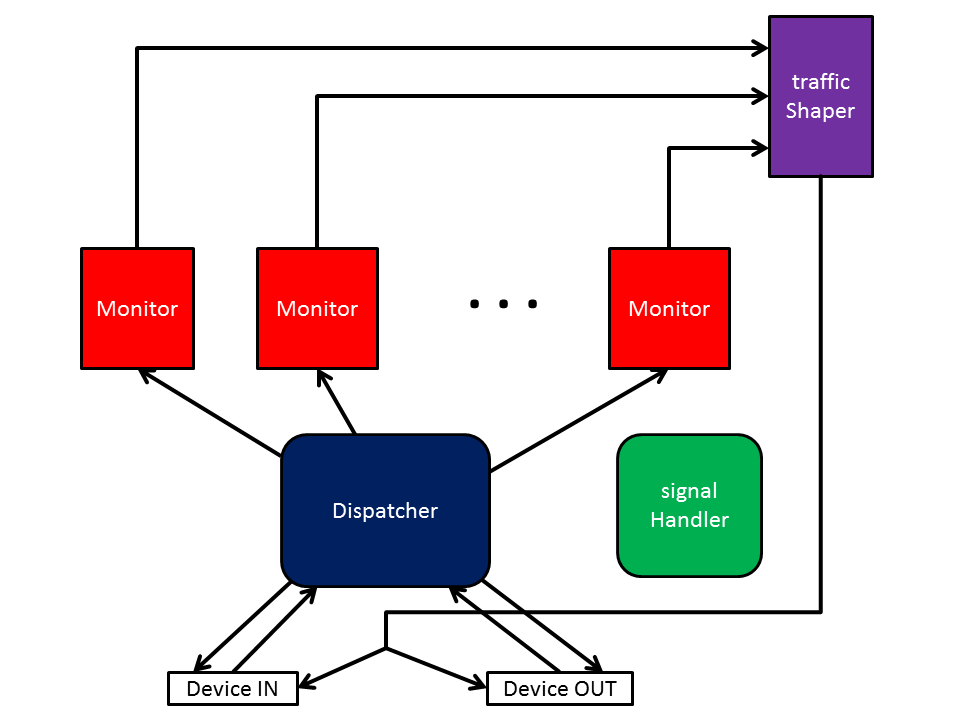
\includegraphics[scale=0.5]{img/arch.png}
\caption{L'architettura del sistema}\label{arch}
\end{center}
\end{figure}

Come si evince dalle considerazioni precedenti, c'è bisogno di una buona potenza di calcolo al fine di gestire grosse quantità di pacchetti.

Poiché l'elaborazione è in un certo senso indipendente da pacchetto a pacchetto, risulta molto potente un'architettura software in cui diversi thread, denominati \emph{monitor}, processano i vari pacchetti di flussi diversi, in modo da sfruttare al meglio i processori multi-core attuali. Il numero di tali thread è definibile come parametro del programma, così da essere flessibile a seconda della macchina su cui si eseguirà il firewall. I compiti del \emph{monitor} sono quelli di aggiungere le informazioni utili nella propria hash table privata, così da evitare meccanismi di lock/unlock piuttosto costosi in termini di tempo, reperire dal gestore delle regole (\emph{ruleManager}) la regola da applicare a quel flusso, ed eventualmente analizzare approfonditamente il pacchetto tramite nDPI (struttura principale privata per evitare ancora meccanismi di sincronizzazione), quindi forwardare o meno direttamente il pacchetto sulla base della regola relativa, o accodarlo nell'apposita coda del thread che si occupa di effettuare lo shaping del traffico. Se tale coda fosse piena, il pacchetto verrebbe scartato per non bloccare l'elaborazione del \emph{monitor}. Insomma, sono questi thread il cuore e la potenza del firewall, non ci si può permettere che perdano tempo.

Per quanto riguarda invece la cattura dei pacchetti, per evitare lock/unlock sui device, si è scelto di mettere un unico thread in lettura da entrambe le schede di rete. Tale thread \emph{dispatcher} forwarda direttamente il pacchetto se si tratta di traffico non-IP o non è trasportato su TPC o UDP (i protocolli applicativi più significativi utilizzano tali protocolli a livello di trasporto), altrimenti mette in coda al thread \emph{monitor} relativo un puntatore ad una struttura contente la copia del pacchetto da processare, insieme ad altre informazioni d'utilità (ad esempio gli IP sorgente e destinatario, le porte, il timestamp del pacchetto, \dots). Ciò è ottenuto riempiendo in modo circolare un array di queste strutture creato durante la fase di inizializzazione del programma, così da non dover far continuamente delle allocazioni dinamiche di memoria, e a grandezza impostabile dall'utente. Quindi avendo le code di comunicazione tra  \emph{dispatcher} e \emph{monitor} un solo produttore e un solo consumatore, possono essere gestite senza l'uso di lock/unlock sui puntatori, garantendo così maggior velocità. Se tale coda fosse piena, il pacchetto verrebbe scartato, così da non bloccare mai il \emph{dispatcher}.

Una volta processato del tutto il pacchetto da parte del \emph{monitor} (ma possibilmente anche del \emph{trafficShaper}), lo slot viene marcato come libero (era precedentemente stato marcato come occupato dal \emph{dispatcher}). Ciò avviene tramite l'uso di operazioni atomiche che, seppur più costose in termini di tempo rispetto alle operazioni normali, permettono di evitare meccanismi quali lock/unlock, che sarebbero ancora più deleteri per le prestazioni.

Ovviamente l'applicazione ha bisogno di un thread che si occupi solamente di inviare i pacchetti sulla base della priorità della coda in cui si trovano. Si è scelto di denominarlo \emph{trafficShaper}.

Per garantire robustezza al programma, tutti i thread mascherano i segnali, tranne un thread (\emph{signalHandler}) usato appositamente per la gestione dei segnali ricevuti, come quello per l'aggiornamento delle regole del firewall o la richiesta di chiusura dell'applicazione.

Da notare infine come l'architettura scelta (illustrata in figura \ref{arch}) non permetta l'esecuzione in zero-copy, cioè senza fare almeno una copia del pacchetto, in quanto c'è bisogno di averne una affinché venga processato e quindi scartato o inviato, il tutto tra le diverse entità del sistema (\emph{dispatcher}, \emph{monitor} e \emph{trafficShaper}). Questo aspetto purtroppo introduce un elemento di degrado delle prestazioni, poiché effettuare una \emph{memcpy} di ogni pacchetto è costoso in termini di tempo.

Tale limitazione si sarebbe potuta evitare con un'architettura diversa, ma meno scalabile e con numerosi punti di sincronizzazione che ne degraderebbero le performance.

Per dare un'idea, tale architettura sarebbe stata con 2 soli thread, uno per scheda di rete, che avrebbero letto e processato i pacchetti (quindi anche inviati o meno), ma avrebbero dovuto usare la stessa tabella hash e la stessa struttura principale per il riconoscimento del protocollo applicativo, dovendo quindi utilizzare delle lock/unlock.

Si è valutata anche la possibilità di utilizzare degli algoritmi detti \emph{lock-free} e \emph{wait-free} \cite{lfpdp,fwsds}, basati su operazioni atomiche quali la \emph{CompareAndSwap} (in sigla, CAS), studiati appositamente per evitare meccanismi di sincronizzazione e attese indefinite per l'operazione da eseguire, al fine di attenuare questo aspetto. Purtroppo queste classi di algoritmi hanno la caratteristica di produrre attesa attiva, che ha un pessimo impatto dal punto di vista dell'uso della CPU che sarebbe continuamente intorno al 100\% di utilizzo.

Inoltre, dovendo utilizzare del tempo anche per analizzare il pacchetto, avrebbero sicuramente fatto più fatica a star dietro ai ritmi dei pacchetti ricevuti dal device di rete, avendo quindi numerose perdite.

A seguito di tutte queste considerazioni, il progetto di architettura qui brevemente discussa è stato accantonato.

\section{Gestione dei flussi}\label{impl-fht}

La flowHashtable, realizzata come classe C++, è la struttura dati designata ad ospitare tutti i vari dati sui flussi che via via i \emph{monitor} si troveranno a dover processare. Ricalca il modello standard visto anche al corso di Algoritmica, ma ha delle peculiarità importanti, essendo studiata per garantire ottime performance per eseguire soprattutto l'inserimento e l'aggiornamento dei flussi, le due operazioni cardine da eseguire per ogni pacchetto ricevuto.

Il primo approccio scelto è stato quello di definire preferibilmente funzioni da usare il più brevemente (3-4 righe di codice) e semplicemente (niente cicli) possibile, così da poterle dichiarare come \emph{inline}. Tale direttiva permette di avere codice replicato a tempo di compilazione, ovunque la funzione sia usata, similmente all'uso delle funzioni macro, ma avendo anche il controllo dei tipi. In termini di prestazioni, questo significa non avere l'overhead di chiamata a funzione e una miglior ottimizzazione del compilatore.

Volendo lavorare su flussi di comunicazione, è stata scelta una funzione hash bidirezionale, anch'essa \emph{inline}. Per realizzarla è stata fatta semplicemente la somma dei campi riguardanti una chiave di flusso, ovvero gli indirizzi IP sorgente e destinazione, le porte, la versione IP e il protocollo di trasporto (TCP o UDP). La chiave di flusso è quella utilizzata per distinguere i vari flussi che vadano a finire nella medesima lista di trabocco, ed è tenuta in modo ordinato sugli IP, coerentemente con le porte, così da garantire una maggior velocità nella comparazione tra chiave e chiave (realizzabile quindi tramite una semplice e veloce \emph{memcmp}).

A livello algoritmico, un accorgimento che consente di ottenere migliori prestazioni, è quello di portare in testa alla lista di trabocco il flusso appena aggiunto o aggiornato. Così facendo, i flussi che hanno frequente scambio di pacchetti possono essere ritrovati prima, mentre i flussi che producono meno traffico, o che sono già terminati, si troveranno in fondo.

Questo semplice accorgimento quindi permette anche di interrompere la ricerca di un flusso in una lista, non appena si trovi un flusso più vecchio di un tempo sufficiente a considerarlo terminato (ad esempio si è scelto un tempo pari a 120 secondi). Questo flusso quindi farà da limite tra quelli attivi e quelli inutilizzati, che potranno quindi essere riciclati per fare spazio ai nuovi flussi in arrivo da aggiungere in lista.

Se né la ricerca né il riciclo vanno a buon fine, allora si procede alla creazione vera e propria di una nuova struttura per contenere il nuovo flusso da monitorare.

Ciò aiuta a migliorare le prestazioni a tempo di esecuzione, evitando di fare continuamente delle chiamate all'operatore \emph{new}. Richiedere al sistema operativo un nuovo segmento di memoria è piuttosto degradante per le prestazioni in quanto c'è bisogno, tra le altre cose, di effettuare un cambio di contesto tra user space e kernel space.

Ma se si facesse solo così, i flussi non sarebbero mai veramente cancellati tramite una chiamata all'operatore \emph{delete}, e quindi lo spazio occupato in memoria sarebbe destinato solo ad aumentare.

Per eliminare questo aspetto critico, si è deciso di creare una funzione apposita da chiamare periodicamente per scandagliare un certo numero di liste della tabella hash per volta, al fine di rimuovere i flussi inutilizzati. Tale numero è fissato ad un decimo della dimensione della tabella, mentre quest'ultima è impostabile dall'utente tramite riga di comando (ma arrotondata alla potenza di 2 più vicina per ragioni di allineamento alla memoria e per sfruttare l'operazione di \emph{and bit a bit} nel calcolo dell'hash, così da velocizzarlo). Se però, il numero di flussi nella  tabella è minore di un certo limite (fissato a 2 volte la dimensione), allora la funzione ritorna immediatamente. Questo è fatto per mantenere anche a regime un certo numero di flussi immediatamente riutilizzabili.

Un altro accorgimento preso che ha sempre a che fare con la dimensione della tabella hash, è quello di dare un numero massimo ai flussi presenti, fissato a 3 volte la dimensione impostata. Questo fa in modo che la memoria non venga occupata fino a saturazione, garantendo quindi anche una prima protezione contro attacchi DoS via flooding.

Da un punto di vista di dati utili salvati per i vari flussi, abbiamo il numero di pacchetti e byte inviati dai due estremi della comunicazione, il timestamp dell'ultimo pacchetto inviato dalla sorgente e dal destinatario, il protocollo applicativo riconosciuto per quel flusso (o l'indicazione di sconosciuto altrimenti),  le precedenti informazioni per il riconoscimento del servizio, e una copia della regola da applicare a quel flusso, comprensiva degli eventuali indici delle code dove mettere i pacchetti per il \emph{trafficShaper}.

Tutte queste informazioni salvate garantiscono uno pieno controllo su ogni flusso, quello che deve avere ogni buon firewall.

Ad esempio, con qualche semplice controllo, sarebbe possibile determinare se un certo flusso sta generando troppo traffico, troppo poco, o sta comunque avendo un comportamento inatteso, e dando quindi la possibilità di intraprendere una particolare azione a fini di sicurezza, come il bloccare tutti i successivi pacchetti.

\section{Gestione delle regole}

Il ruleManager è il componente del sistema che si occupa della gestione delle regole. Anch'esso è scritto in C++ e studiato per garantire le migliori performance e minor occupazione in memoria.

Sfrutta due strutture dati per svolgere il suo compito. Una è una semplice lista delle regole vere e proprie, l'altra è un albero binario che contiene in ogni nodo un puntatore alla regola nella lista da applicare. Ovviamente c'è la possibilità che alcuni nodi non contengano alcuna regola.

Quest'ultima struttura dati è utilizzata anche per le tabelle di routing ed è anche conosciuta come \emph{Patricia Trie} \cite{trie}.

L'albero e la lista sono costruiti sulla base di un file XML (un esempio ne è il codice \ref{esconf}) contenente le regole e specificato come input del programma.

Col tag principale \emph{ruleSet} si specificano i comportamenti di default nel caso non si trovino regole associate ad un certo IP (neanche sulla base del \emph{prefisso più lungo}). Tramite i tag figli \emph{rule} è possibile specificare una nuova regola impostando l'id, l'azione da eseguire (se consentire o negare) e la lista dei protocolli a cui applicare l'azione specificata, creando poi l'elemento relativo nella lista.

Con i tag figli \emph{match\_v4} e \emph{match\_v6} è possibile impostare per un certo IP (o sottorete, scritta nell'usuale notazione CIDR), l'id della regola da utilizzare (tradotto dal programma nel relativo puntatore), creando (se necessario) i nodi nell'albero. Quindi una data regola è riutilizzabile in più \emph{match}.

La lista dei protocolli specificabile in \emph{rule} merita una piccola spiegazione.

Naturalmente è possibile utilizzare la parola chiave \emph{ALL} per indicarli tutti, ma è anche possibile fare una lista, intervallata da spazi, coi nomi dei protocolli desiderati (ad esempio, \emph{dns dhcp http dropbox}). Dopo ogni protocollo applicativo è inoltre possibile specificare (mediante @ e l'indice) la coda del trafficShaper dove accodare eventualmente il pacchetto per quel servizio (ad esempio, \emph{dns@3 dhcp@8 http dropbox@2}). Questa stringa di protocolli sarà quindi convertita in due strutture. Una è una bitmask nella quale ogni bit rappresenta un protocollo (se 0 il servizio sarà da bloccare, altrimenti da far proseguire). L'altra è un semplice array in cui ogni posizione rappresenta l'indice della coda nella quale accodare eventualmente i pacchetti del relativo servizio (ricordiamo che ad ogni servizio riconosciuto dalla libreria nDPI è associato un intero univoco, utilizzato quindi come indice dell'array).

Per quanto riguarda la ricerca di una regola, purtroppo da un punto di vista algoritmico non c'è molto da fare. Bisogna scendere giù per i nodi dell'albero binario, scegliendo se andare al figlio 0 o al figlio 1 in base ai bit dell'indirizzo IP, e reperire la regola dal puntatore immagazzinato nel nodo relativo all'esatto match con l'IP o all'ultimo nodo con una regola valida incontrato, che è l'applicazione più naturale per trovare la corrispondenza sul prefisso più lungo.

Questa operazione ha un limite superiore per quanto riguarda la complessità, infatti sono necessari al massimo 32 (128 per l'IPv6) cicli per trovare la regola per un dato IP. Doverla ricercare per ogni pacchetto processato sarebbe comunque poco desiderabile a tempo d'esecuzione, così si è scelto di immagazzinare nella tabella hash una copia della regola trovata.

Come tutti i firewall degni di tale nome, il ruleManager deve permettere l'aggiornamento delle regole anche durante l'esecuzione delle normali attività.

Si è quindi deciso di implementare una funzione da chiamare al fine di computare tale aggiornamento. In questo caso, ogni volta che al programma venga inviato un segnale di tipo SIGUSR1, si richiama tale funzione.

Essendo una fase delicata e non volendo introdurre meccanismi di sincronizzazione, viene eseguita in più passi.

Per prima cosa viene controllato che dal precedente aggiornamento sia stata chiamata un'altra funzione apposita per liberare lo spazio occupato dalle vecchie strutture.

Se è effettivamente così, allora vengono salvati i vecchi puntatori alla lista e all'albero correnti.

Inizia quindi un nuovo processo di parsing del file XML di configurazione, già specificato all'avvio del programma, al fine di costruire una nuova lista e un nuovo albero, mediante puntatori temporanei. Se tale costruzione riesce (notiamo che per farla fallire non dovrebbe essere specificato il tag principale \emph{ruleSet}, quindi una condizione abbastanza limite), allora i due nuovi puntatori vengono inseriti al posto dei due principali, altrimenti vengono ripristinati i puntatori alle vecchie strutture dati prima salvate.

Infine viene aggiornato un semplice intero contatore che identifica la versione delle regole attuali.

Questo contatore sarà utilizzato anche dai \emph{monitor} al fine di stabilire se la regola salvata nella propria hash table è aggiornata rispetto alla versione del ruleManager.

L'approccio descritto permette, seppur con un temporaneo aumento di memoria occupata, di evitare meccanismi di sincronizzazione. Notiamo infatti che se durante le operazioni di aggiornamento dovesse arrivare una richiesta per la ricerca di una regola, verrebbe utilizzato il puntatore all'albero principale e non quello temporaneo ancora in via di costruzione. Solo una volta finita l'operazione il nuovo puntatore viene copiato al posto di quello principale.

Starà poi al chiamante cancellare le precedenti strutture dati. In questo caso si è scelto di farlo in automatico via \emph{signalHandler} dopo un paio di secondi, in seguito alla ricezione di un segnale di tipo SIGALRM impostato con una chiamata alla funzione apposita \emph{alarm}.

\section{Il sistema garante del QoS}

Il trafficShaper è un altro componente essenziale del firewall. Realizzato come classe C++, permette di fare lo shaping del traffico.

La sua configurazione avviene all'avvio del programma tramite lo stesso file XML di configurazione contenente le regole (un file d'esempio è riportato di seguito nel listato \ref{esconf}). A differenza di esse però, non è possibile modificare nulla durante tutta l'esecuzione.

Si possono specificare il numero e la capacità delle code da creare (nel tag \emph{queueSet}), e naturalmente l'id e il peso in kByte (che verranno inviati al secondo) di ogni coda (nei tag figli \emph{queue}).

Internamente è formato da qualche variabile di stato, come l'ultima coda visita, ma soprattutto da un certo numero di code, dette \emph{masterQueue}. Ognuna di esse ha al suo interno varie informazioni e la coda vera e propria, dove ogni \emph{monitor} cercherà di mettere il puntatore alla struttura (ricevuto dal \emph{dispatcher}) contenente il pacchetto da inviare.

Questa operazione è eseguita attraverso la chiamata alla funzione \emph{enqueue}, che prende chiaramente come parametro il puntatore alla struttura contenente il pacchetto e la coda dove inserire tale puntatore, ed avviene in mutua esclusione, poiché può essere eseguita da più thread contemporaneamente. Notiamo come questa operazione, seppur semplice, costituisca un collo di bottiglia, dovuto alla concentrazione di richieste critiche e quindi all'uso di lock/unlock.

L'operazione cardine però che costituisce il vero cuore dello shaper è la \emph{dequeue}, che ricerca il prossimo pacchetto da inviare e ne restituisce il puntatore. Notiamo fin da subito che questa funzione può essere eseguita senza mutua esclusione, in quanto fatta da un unico thread.

La scelta è ricaduta su un semplice algoritmo di shaping denominato \emph{token bucket} \cite{tba}. Tale algoritmo consiste in pochi e semplici passi.

Le \emph{masterQueue} sono gestite in modalità (Deficit) Round Robin \cite{drr}, così da garantire un buon grado di equità (\emph{fairness}). Ad ogni visita di una \emph{masterQueue}, le vengono attribuiti un certo numero di \emph{token} calcolati in base al tempo passato dall'ultima visita di quella coda e il peso della stessa \eqref{calccrediti} e sommati ai precedenti, ma limitati al massimo al peso della coda \eqref{calctoken}.

\begin{equation}\label{calccrediti}
\textit{crediti} = {\textit{peso della coda}} * {\textit{tempo passato}}
\end{equation}
\begin{equation}\label{calctoken}
\textit{token} = \begin{cases} \textit{token} + \textit{crediti}, & se \leq \textit{peso della coda} \\ \textit{peso della coda}, & altrimenti\end{cases}
\end{equation}

Se i \emph{token} sono in numero maggiore o uguale alla lunghezza del pacchetto puntato dalla \emph{head} della coda, allora tale pacchetto può essere inviato e ne vengono scalati i \emph{token} necessari, altrimenti, si procede con la coda successiva da esaminare.

Nell'improbabile ipotesi in cui tale ciclo non trovi alcun pacchetto da inviare girando tutte le \emph{masterQueue}, ci si sospende per un microsecondo e poi si ricomincia. Questo approccio è stato scelto perché permette una miglior reattività dello shaper.

Come si può ben capire, è un componente piuttosto semplice, ma svolge appieno il suo ruolo.

Un aspetto comunque molto importante è l'efficienza del calcolo del tempo. Se si usasse una funzione come la \emph{gettimeofday}, si avrebbero performance peggiori, in quanto la sua esecuzione consta di diverse operazioni che coinvolgono anche il kernel. Così si è optato per l'utilizzo intelligente del contatore dei cicli di clock del processore, letti tramite la chiamata alla semplice funzione assembler \emph{rdtsc} \cite{rdtsc}. Nella fase di inizializzazione viene calcolata la frequenza stimata del processore, che verrà poi usata ogni volta che ci sia bisogno di calcolare il tempo passato in un intervallo di cicli di clock, come da naturale relazione di seguito riportata \eqref{calct}.

\begin{equation}\label{calct}
\textit{tempo passato} = \frac{\Delta\textit{ cicli di clock}}{\textit{frequenza CPU}}
\end{equation}

\clearpage
\lstinputlisting[language=XML,caption={Una semplice configurazione d'esempio},label=esconf,frame=single,rulecolor=\color{black},basicstyle=\tiny,showstringspaces=false,breaklines=true,morekeywords={confFile,queue,queueSet,rule,ruleSet,match_v4},keywordstyle=\color{blue},stringstyle=\color{green}]{codice/exampleConf.xml}